\section{Sistema internazionale S.I.}

Diamo la seguente definizione:
\begin{grf}
	Una grandezza fisica è una proprietà di un corpo che si può misurare oggettivamente (nel senso che chiunque la misuri deve ottenere lo stesso risultato).
\end{grf}
 Consideriamo la prima grandezza che incontreremo nello studio della meccanica, la lunghezza. Per definire una grandezza fisica, occorre darne una definizione operativa, ossia definire \textit{come si misura}, fornendo un procedimento e una unità di misura. Nel caso della lunghezza, si utilizza un righello (o un metro da falegname) che è un oggetto rettilineo sul quale sono indicate delle tacche. Le tacche riportano l'unità di misura ripetura tante volte. Ad intervalli regolari, la scala così costruita, contiene tacche più grandi utili per calcolare la cosiddetta sensibilità dello strumento ossia, \textbf{la più piccola variazione di una grandezza che uno strumento può rilevare}. Nel caso della  figura \ref{fig:lun} la misura della lunghezza del lato del tavolo, si scrivedrà:
 \[
 L=\SI{0,763}{\meter} =\SI{763}{\milli\meter}
 \]
 
    \begin{figure}[h!]
    \centering
    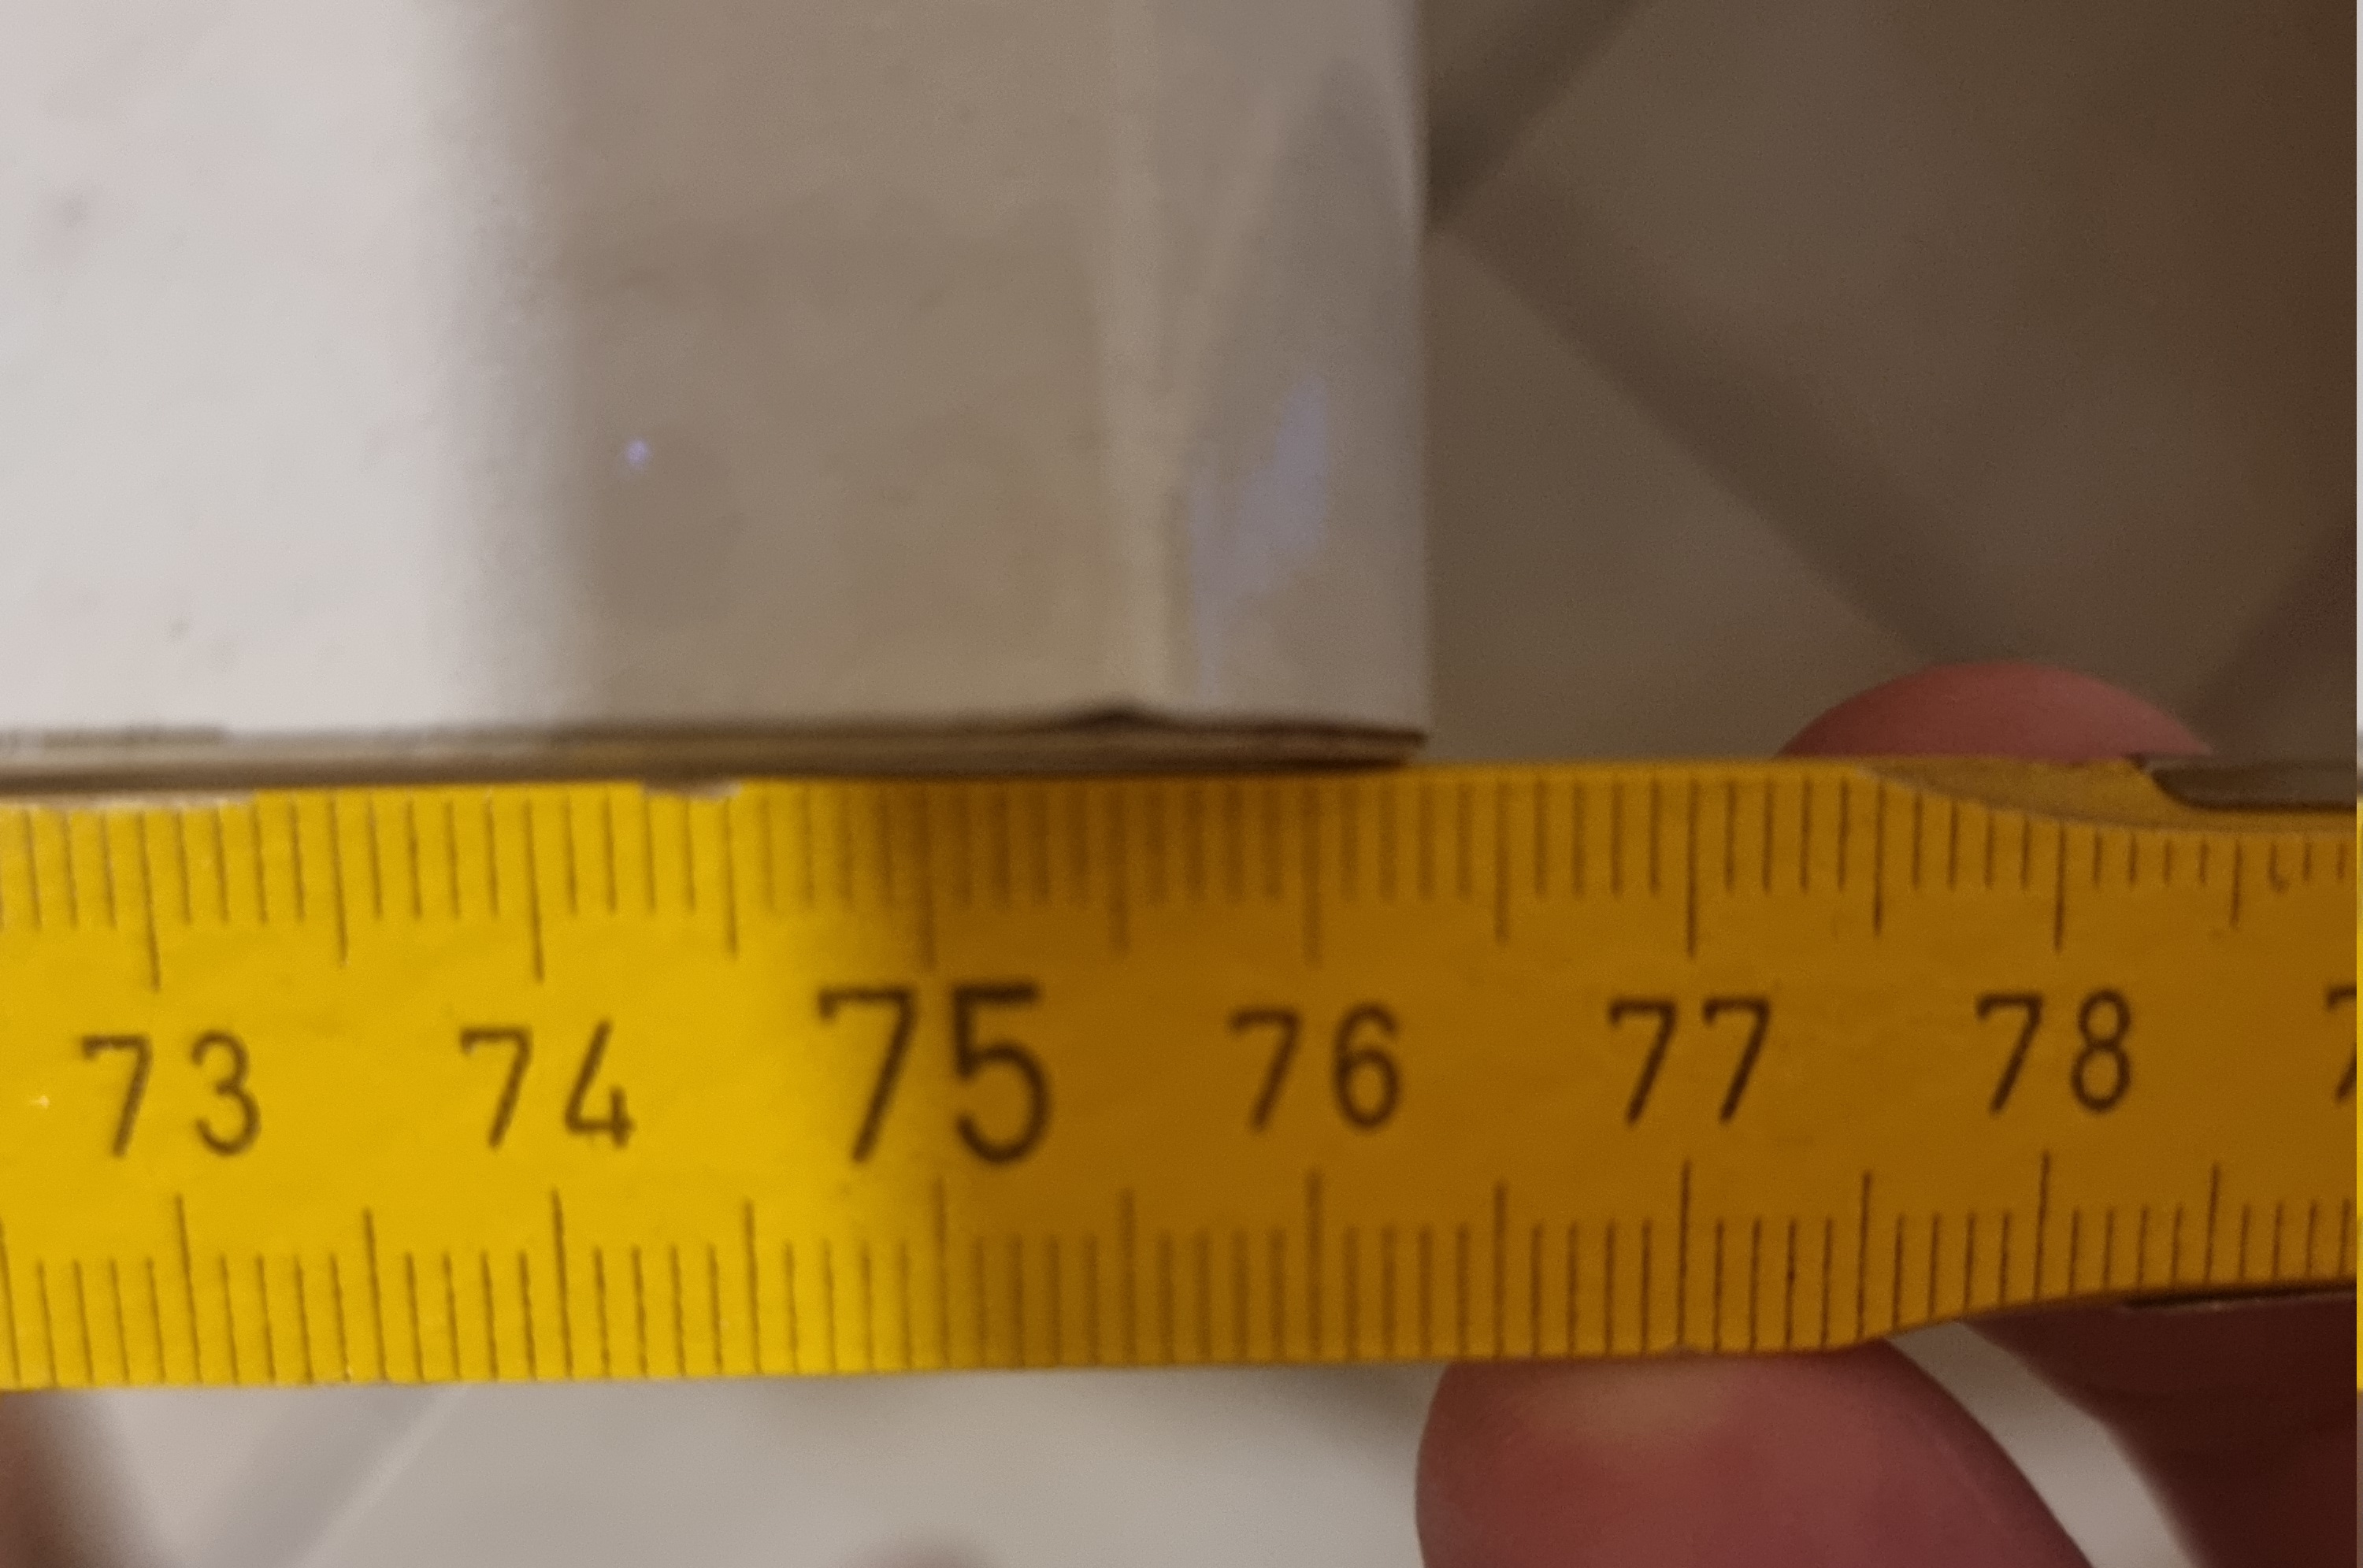
\includegraphics[width=0.5\linewidth]{path_to_image/lun.jpg} 
    \caption{Misura di lunghezza col metro da sarto}
    \label{fig:lun}
\end{figure}  
 
Questa misura, indica chiaramente che abbiamo un ``errore'' di un millimetro (vedremo più avanti cosa sono gli errori) ossia, siamo certi che la nostra misura è compresa nel seguente intervallo:
\[
\SI{762}{\milli\meter} \le L \le \SI{764}{\milli\meter}
\]


Uno strumento di misura è uno strumento tarato, ossia uno strumento che ci fornisce direttamente  il valore di  una misura rispetto ad una certa unità di misura. Ad esempio, lo strumento che abbiamo usato per misurare il lato del tavolo, si chiama "metro da falegname" ed ha tacche distanti tra loro 1 mm. Questo strumento misura la lunghezza, ma esistono altre grandezze fisiche e quindi altri strumenti. Nella tabella \ref{tab:si_units} elenchiamo le grandezze fondamentali del cosiddetto sistema internazionale (abbreviato S.I.) un insieme di 7 grandezze che un comitato tecnico scientifico ha approvato in modo da semplificare ad esempio i commerci e la comunicazione scientifica poiché al mondo, in ambiti e paesi diversi, erano e sono tutt'ora in uso, unità diverse (nei paesi anglosassoni ad esempio, sopravvivono unità come pollice, piede, oncia, miglia, gallone etc.). Per questo corso ci serviranno il primo anno solo le prime quattro (lunghezza, massa, tempo, temperatura). Per quanto riguarda la temperatura, useremo quest'anno il grado centigrado, simbolo °C. 

\begin{table}[h!]
	\centering
	\begin{tabular}{|c|c|c|}
		\hline
		\textbf{Nome della Grandezza} & \textbf{Simbolo} & \textbf{Strumento di Misura} \\
		\hline
		Lunghezza & m & Metro a nastro, righello \\
		\hline
		Massa & kg & Bilancia \\
		\hline
		Tempo & s & Orologio, cronometro \\
		\hline
		Intensità di corrente elettrica & A & Amperometro \\
		\hline
		Temperatura termodinamica & K & Termometro \\
		\hline
		Quantità di sostanza & mol & Contatore di particelle (spesso teorico) \\
		\hline
		Intensità luminosa & cd & Fotometro \\
		\hline
	\end{tabular}
	\caption{Grandezze fondamentali del Sistema Internazionale con simboli e strumenti di misura.}
	\label{tab:si_units}
\end{table}

Come avrete notato, il valore di una grandezza si scrive usando una lettera, nel nostro caso la L. Non bisogna confondere le lettere usate per la misura con le lettere usate per l'unità di misura. Ad esempio nella scrittura $m=\SI{4}{\kilo\gram}$, emme è il simbolo della grandezza. Nella scrittura $L=\SI{10}{\meter}$, la emme significa "metro" ed è l'unità di misura.

